\documentclass[journal]{IEEEtran}

\usepackage{cite}
\usepackage{amsmath}
\usepackage{verbatim}
\usepackage{multirow}
\usepackage[unicode,pdftex]{hyperref}
\usepackage{xcolor}
% \usepackage{setspace}

\ifCLASSINFOpdf
\usepackage[pdftex]{graphicx}
\else
\fi

\usepackage{todonotes} 
\hyphenation{op-tical net-works semi-conduc-tor}

\newcommand{\reffig}[1]{Fig. \ref{#1}}
\newcommand{\refsec}[1]{Section \ref{#1}}
\newcommand{\refeq}[1]{Eq. \ref{#1}}
\newcommand{\reftab}[1]{Table \ref{#1}}

\newcommand{\tabincell}[2]{\begin{tabular}{@{}#1@{}}#2\end{tabular}}
\newcommand{\stodo}[1]{\todo[size=\tiny]{#1}}


\DeclareMathOperator*{\argmax}{argmax}
\DeclareMathOperator*{\argmin}{argmin}


\definecolor{level2}{RGB}{255,255,255}
\definecolor{level3}{RGB}{10,10,10}
\definecolor{revised}{RGB}{100,101,140}
\definecolor{continue}{RGB}{255,0,0}
\definecolor{filltext}{RGB}{0,255,255}

\begin{document}
\title{Deep Variation Transformation for Foreground Detection}

\author{Yongxin Ge, 
        Xinyu Ren, 
        Chenqiu Zhao,
        Anup Basu
        \thanks{Yongxin Ge is with School of Software Engineering, Chongqing University, Chongqing (401331), PR China.}
        \thanks{Xinyu Ren is with School of Software Engineering, Chongqing University, Chongqing (401331), PR China.}
        \thanks{Chenqiu Zhao is with Department of Computing Science, University of Alberta (T6G 2E1), Canada.}
        \thanks{Anup Basu is with Department of Computing Science, University of Alberta (T6G 2E1), Canada.}
        }


% \authorrunning{Lecture Notes in Computer Science: Chongqing University}


\maketitle


% \begin{spacing}{2.0}
\begin{abstract}
%
% 运动检测的已有方法主要关注于像素值的变化。
Previous approaches to foreground detection generally analyzed the variation of pixel observations.
% 本文中,我们分析了像素的变动,并提出了DPVTL方法。
% In this paper, we focus on transforming the variation into a new space where that there is an obvious difference between the patterns of variation produced by the moving objects and the background,
In this paper, we focus on transforming the variation into another space where the entry of variation is easily classified, using a novel foreground detection method called Deep Pixel Variation Transformation Learning (DPVTL).
% 一个FCN被用来寻求一个变换,可以使变换过后的像素值线性可分。
% 具体来说,我们用一段像素观测值表示pixel variation,并用作网络的输入。 
    In particular, the pixel variation is represented by the sequence of pixel space, which is used as the input to a fully convolutional network space (FCN) to find a transformation of pixels' variation.
% 接下来,FCN学习像素变动的模式,并接上一个线性分类器给像素打标签。
Then, the FCN is trained to learn the pattern of pixel variations for the transformation, followed by a linear classifier for labeling the pixels as foreground or background.
%    
% XXX 这句话还是有点问题
% 这句话我也没看懂。。。
Resulting from the global analysis of pixel variations and the strong learning ability of deep learning networks,
the proposed approach adaptively learns a good transformation from pixel variations to label and generate good performance in diverse natural scenes.
%    \textcolor{red}{
% Benefited from the ingenious utilization of deep learning network leading by our clear cognition of essence about foreground detection problem,
%    the proposed approach adaptively generates superior performances in diverse nature scenes.}
%
Comprehensive experiments on several standard benchmarks demonstrate the superiority of the proposed approach compared to state-of-the-art deep learning and traditional methods.
%
\end{abstract}

\begin{IEEEkeywords} 
    foreground detection, Feature Transformation, Deep Learning,
\end{IEEEkeywords}

\IEEEpeerreviewmaketitle

\section{Introduction}
%背景检测的背景介绍
Foreground detection is a fundamental problem in computer vision\ \cite{Bouwmans201431} that has been approached over decades with an increasing number of cameras.
It is widely used in applications involving video processing \cite{Barnich2011_2011_TIP}.
% 传统的方法是怎么做的,有什么问题
Typically, it is recognized as a binary classification task that assigns a label to each pixel in the video stream,
for either belonging to the background or foreground scene.
Traditional foreground detection algorithms focus on analyzing pixel variations, establishing background models with statistical methods such as GMM\cite{Stauffer1999}\cite{lee2005} and KDE\cite{Elgammal2000Non}\cite{Mittal2004KDE}.
However, due to the unpredictability and speed of pixel variations in natural scenes,
the variation becomes unordered and is hard to analyze for foreground detection.
Therefore, foreground detection is still a challenging problem in complex natural scenes.
% 现有的方法在简单场景中效果很好了
%Existed methods have already achieved well performances in the scenes of low diversity or complexity, such as the indoor scenes.
%
% 8.21 Ren: 你原来讲传统做法的时候是说它们关注与像素的变动,这不对啊,它们明明关注的是像素的分布,我们才更注重于变动。
% 8.21 Ren: 还有我看有人说,论文里面不用加's 可以直接名词拼接,就像这样 pixel variation.  F. 名词修饰:在学术文章中,很多时候会用到直接用名词做修饰,而不用’s 或 ……of …… 的形式。常见的这类词有:reaction rate;reaction rate constant;reaction temperature;reaction condition  molecular weight distribution……
%

% 总而言之,foreground detection依然有很多问题
% 8.21 Ren: 这里有个however,上上句也有个however.......怎么搞啊?
% 8.21 Ren: 改到这里,不知道怎么改了,先更你确定一下吧,variation 跟 distribution 有没有区别?我的理解是variation就是有时间顺序的,之前的方法没有考虑道时间顺序性,所以就不能叫做variation.只能叫distribution.
% 8.21 Ren  我觉得我们应该确定的是,传统统计学的方法只关注数据的分布概率,而我们更多考虑的是数据在时序上的变动。
% 8.21 Ren  因为这一段跟你的理解有冲突,所以先商量后再改吧。


% 第二段重点阐述什么是deep variation learning
% 在多样的自然场景中,前景可能产生和背景相似,甚至相同的像素,而这种像素很难去分析
In diversely natural scenes,
it is possible that moving objects produce similar or even the same observations of pixels compared to the background.
% similar to their counterparts of background but actually belong to foreground .
% 如图所示,像素观测值C就和背景的值几乎一模一样,
As shown in \reffig{idea},
observation C is closely related to the observations which belong to the background. However, it is actually produced by moving objects and should be classified as foreground.
% 大多数情况下,他都会被划分成背景
Unfortunately, in most cases, it is quite possible that C will be falsely classified due to the similarity with counterparts of the background.
% 我们的就是希望把这个variation 转化到更简单的地方去
In this work, we focus on learning the pattern of pixels' variation and transforming the variations into a new space where the observations are easier to classify, rather than learning a classifier for individual pixels.
As shown in the bottom part of \reffig{idea}, the pattern of a fragment consisting of observations A-D can be learned by the network and transformed into another fragment where these observations are easily and correctly classified as foreground.
% transformatin 之后,就很容易分类了,然后这就是我们的方法的核心了
Based on this, the Deep Pixel Variation Transformation Learning model for foreground detection is proposed.
% motivation
% %实际应用中的挑战
% \todo{the main purpose of the second paragraph is showing our idea. But be careful that you should not mention any details of our method which is the content of third paragraph. Pls re-write this part according to figure 1. The main content should be the description of figure 1, as well as our idea, insight}
% Existed methods have already achieved well performances in the scenes of low diversity or complexity, such as the indoor scenes. 
% However, foreground detection is still unsolved because of the complexity and the diversity of natural scenes.
% There are many forms of natrual scenes, for example, camera jitter, dynamic background, bad weather, illumination changing, intermittent object motion\cite{CDN2014}. In these situations, the backgrounds are no longer being static, while in fact, the background can be dynamic and complex, which brings some severe challenges to the traditional methods.
% To solve this problem, we bring up a novel conception of variation transformation, wherein the historical observations of each pixel are conceived as a unity, the pixel variation. Each piece of pixel variation contains the complete temporal information of historical observations, which turns out to be our advantage that not only the distribution of observations, but also the temporal coherence plays an important role in the task.
\begin{figure}[!t]	% FIGURE: figure/fig1 
\centering
    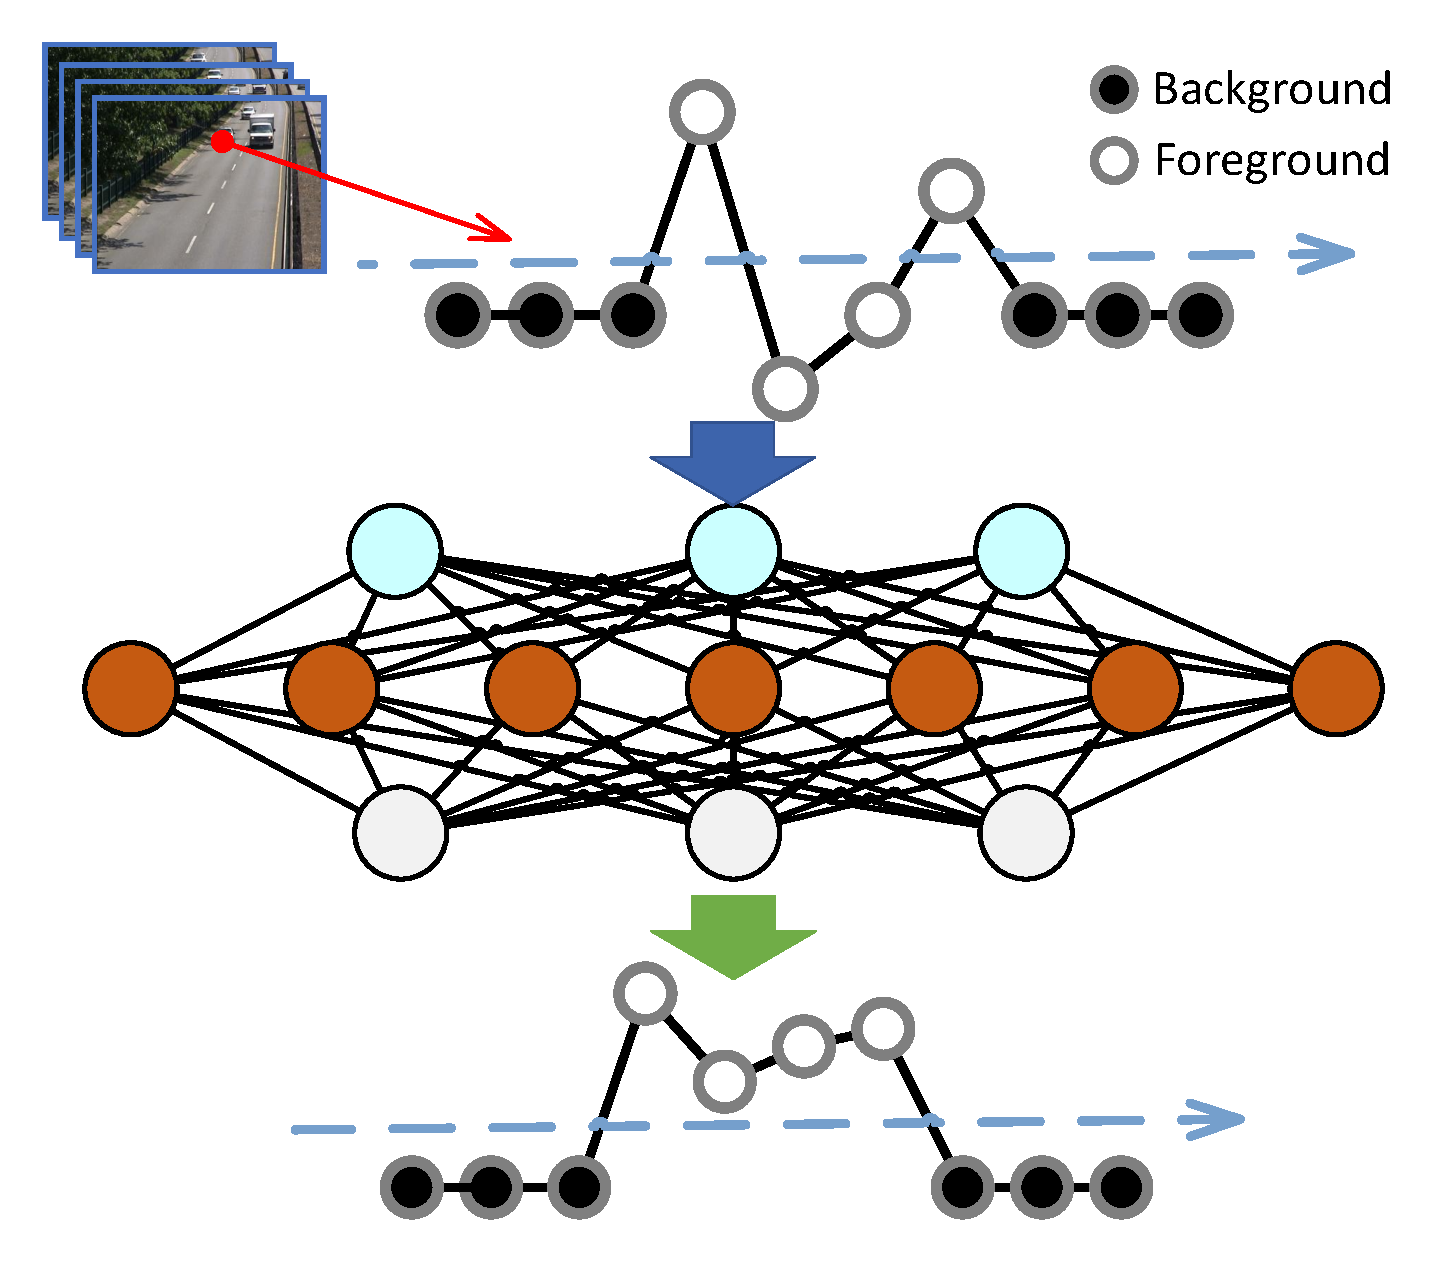
\includegraphics[width=\linewidth]{figure/demo.pdf}
    % 图例里描述一下。
    \caption{Demonstration of deep variation transformation. Due to the complexity of natural scenes, the original pixels' variation is hard to classify correctly. After transforming by a deep learning network, the pixels in variation become easy to be correctly classified as foreground and background correctly.}
    \label{idea}
\end{figure}
%The demonstration of deep variation transformation. The pixels in the transformed variation become easier to be classified as foreground and background correctly
%本文的想法和优势
% The previous methods have already made great progress in generating some sophisticated background models with given videos. 
% Unfortunately, some instructive clues have been long put aside and neglected, since there is no efficient way to deal with them. 
% For instance, the statistical methods\cite{Stauffer1999} model the pixel-wise distribution of historical observations over time, while having no concerns over the sequential information in a video stream. 

%具体介绍
% XXX 一句话,换一行!!!
% In this paper, we propose a novel Deep Variation Transformation Learning (DPVTL) model for foreground detection in diversely natural scenes. 
In the DPVTL model, 
the sequence of pixel observations is used to represent the variations and input into the network for learning,
which encodes both the intensity distribution and the sequential information.
%
Then, a Fully Convolutional Network (FCN)\ \cite{Shelhamer2017fcn} is applied to learn patterns of pixel variations and find a transformation which guarantees the linear separability of pixels in the transformed variation.
%
In particular,
we take advantage of the strong learning ability of deep neural networks to learn an end-to-end representation of the pixel variation in a new space where they can be easily classified as background or foreground.
%
Utilizing the innovative framework of variation transformation,
the proposed approach works well for a diverse range of complex scenes.
% in diverse complex scenes adaptively.
%
%Moreover,
%since the pixel sequences are extracted from individual pixels, a large number of pixel patches may be extracted from only a single image stack, which promises that sufficient training data can be obtained with limited groundtruth.
% 
% 
% 
% \todo{This paragraph is too short! provide comprehensive details of our work!}
% % The final prediction can be obtained by thresholding of the transformed variation. 
% %Our contributions can be summarized as follows:
% The contridbutions of proposed approach is shown as follows:
% \begin{itemize}
% \item We proposed the pixel observation patch to describe the pixel variation, which encode both the intensity distribution and sequential information over time.
%     The observation patch is obtained by reshaping the vector of a pixel's historical observations, subtracted from the image stacks. 
% \item We propose a deep neural network for variation transformation. 
%     Our FCN network is trained to learn the pixel variation and generate a new representation in a new feature space. 
% \end{itemize}
% 
%文章结构

%The outline of this paper is as follows: In Section II, we give a brief discussion about the early and recent relevant works. 
% XXX 不会用引用可以问我或者曲师兄。
The rest part of this paper is organized as follows: In \refsec{sec2}, we briefly discuss both early and recent relevant literature. 
%
Details on the variation transformation are presented in \refsec{sec3}. The architecture of the network is introduced in \refsec{sec4}, This is followed by experiments and comparison results in \refsec{sec5}, before concluding the paper in \refsec{sec6}. 
% \todo{please revise this part by using command refsec}

\section{Related Work}
\label{sec2}
Over the last few decades, a large number of foreground detection methods have been proposed,
which are broadly categorized into pixel-based, region-based and learning-based methods.
\subsection{Pixel-based methods}
% Ren:重新解释了pixel based methods
Pixel-based methods usually assume the independence between neighboring pixels,
and utilize low-level features, such as color or gradients for background subtraction.

%GMM 
% cqzhao: 我没有看到过over time,如果你在trans或者顶会(ICCV,CVPR,ECCV)里找到了论文原话,那你可以用哦。
In particular, the Gaussian Mixture Model (GMM) proposed by Stauffer et al.\ \cite{Stauffer1999} is the most popular approach among pixels-based methods\cite{Goyal2018}.
% 注意英语和汉语的表达习惯
It utilizes a mixture of weighted Gaussians to model the probability distribution of each pixel over a time sequence.
%
Pixels are considered as background when the probability generated by Gaussians are higher than a user threshold.
% \textcolor{red}{Pixels are considered as background if there exists a Gaussian function includes their values with sufficient evidence.} 
%GMM+i
Zivkovic et al.\ \cite{Zivkovic2004} improved the GMM method by utilizing a recursive equation
to automatically update the parameters and adjust the number of components of the mixture needed for each pixel. 
%
%codebook
Kim et al.\cite{Kim2005} presented the codebook method, which records the sampling background values on codewords for each pixel position.
The incoming pixels are compared with these codewords to see if their distances lie within a certain bound. 
%KDE
In addition, a non-parametric background model is proposed by Elgammal et al. \cite{Elgammal2000Non}. 
They assume that each background pixel is drawn from a probability distribution function, which is estimated in the Kernel Density Estimation space (KDE). 
%Vibe
Another non-parametric method is proposed by Barnich et al. \cite{Barnich2011_2011_TIP}, called the Visual Background Extractor (ViBe). 
%
The background model of ViBe consists of pixel samples from the video stream. 
%
Each pixel in the current frame is compared with sample pixels from the corresponding background model and labelled as the foreground when there exists sufficient samples with a distance to itself within a certain range. 
%PBAS
To adaptively update the parameters, Hofmann et al.\cite{Hofmann2012Background} improved ViBe by presenting an adaptive threshold, 
which depends on the pixel position and a background dynamics metric.

%提出其他方法的问题,指出他们的缺陷
Unfortunately,
the pixel-based methods ignore the spatio-temporal information due to their assumption of independence between pixels.
But there is, in fact, a strong coherence in image sequences that contain abundant hidden clues for the background model. 
%
%提出我们的改进,我们认为像素在时序上是互相依赖的
% tight interdependence 明明在google scholar里查得到很多用的好不好...
% To address this shortcoming, 在一篇2018的CVPR的摘要里有啊
% “High Quality Estimation of Multiple Intermediate Frames for Video Interpolation”
To address this shortcoming, we introduce a framework of variation transformation learning, 
where a pixel's historical observations are embedded into a piece of pixel patch and sorted in chronological order as a whole for the training of our DPVTL model.
%这样的优点在于保留了数据的完整性,保留了数据的时序相关性。
Bringing together the historical observations ensures data integrity and preserves the temporal coherence of our training data. 
On the other hand, the application of a neural network guarantees strong learning ability of our model.
Thus, the proposed approach is more capable of learning the patterns of pixel variation and exploiting the spatio-temporal context, compared to those classifiers based on the assumption of pixel independence. 
%所以我们方法比基于像素的要好。
%Hence we demonstrate a comparatively better performance in modelling some challenging scenes, like illumination changing and intermittent object motion.
%\todo{you should discuss the difference between the proposed approach and pixel-based method. What is your advantage compared with these previous work? Why they failed and why our method work?}
%
%
%
%
%
%
\subsection{Region-based approaches}
% Ren: 好的好的,不乱吹了,我看过有说have similar values的。。。。
Region-based approaches are usually performed at block-level resolution, in order to exploit the spatial context between neighboring pixels.
%

%(Regularized region-based)
Varadarajan et al.\ \cite{2015_PR_Varadarajan20153488} proposed a region-based GMM model,
which is derived using the expectation-maximization (EM) theory considering neighboring pixels.
% Spatiotemporal GMM
In addition, 
Chen et al. \cite{2017_TPAMI_GANGWANG} combined GMM with constraints on temporal and spatial information from the optical flow and hierarchical superpixels.
%(Bayesian Modeling)
Moreover, 
Sheikh et al.\ \cite{Sheikh2005Bayesian} introduced a framework based on the Markov Random Field modeling with Maximum A Posteriori 
probability (MAP-MRF) estimation, which incorporates the pixel location into background and foreground KDEs for the detection based on spatial context.
%(Robust Foreground Object ICPR2010 Vikas Reddy )
% 这里原文就是用了三层的分类器,不同的方法,一层又一层。
Similarly, in \cite{Reddy2010Robust}, original images are divided into overlapping blocks. Each block is sequentially processed by an adaptive multi-stage classifier, which consists of a likelihood evaluation, an illumination invariant measure and a temporal correlation check.
%( Robust Region-Based ICPR)
Hence, Izadi et al.\cite{Izadi2008Robust} presented a robust region-based approach, which generates a pair of foreground maps based on gradient and color respectively. Any foreground region that does not exist in the first foreground map could be recovered from the other one.

In contrast, we accept the assumption that neighboring blocks of background pixels should follow similar variations over time, 
and combined the pixel variation with its spatial neighbors to revise our prediction. 
Due to the application of deep learning, the proposed approach is more powerful in capturing the structural background variation and achieves significant improvement compared to its competitors.
%
%
%
% \subsection{learning-based methods}
\subsection{Machine Learning based Methods}
The last category of background subtraction methods applies traditional machine learning and deep learning for foreground detection.

%
%SVM
Traditional machine learning methods are commonly involved with support vector machines (SVM)\cite{Chen2011}\cite{Han2012} and Bayesian methods\cite{Sheikh2005Bayesian}\cite{2012_TIP_OP_6099616}\cite{Zhang2014Statis}. 
For example, Han et al. \cite{Han2012} integrated gradient, color, and Haar-like features to address the spatio-temporal variations for each pixel. 
Their background model is obtained for each feature in a kernel density framework and a SVM is employed for classification.

%
In recent years, deep learning methods have begain began to flourish in several computer vision fields, 
and have demonstrated effective capabilities to handle time-series problems\cite{Mobahi2009}\cite{LANGKVIST201411}. 
%
A novel approach for foreground detection with the use of the Convolutional Neural Network (CNN) is proposed by Wang et al.\cite{wang2016PRL}.
They utilize a CNN with a cascade network architecture for segmentation in foreground detection, which performs very well with sufficient training data.
%
% Ren: 这里我解释一下,为什么看上去这么冗余。这家伙先自己用中值滤波求了个平均背景,然后把平均背景 patches 跟对应的origin image patches 组合作为网络输入,他训练的groundtruth也可以来自其他比如GMM的分类结果图。
Braham et al. \cite{Braham2016deep} employed a scene-specific CNN, 
which is trained with corresponding image patches from the background image, video frames and groundtruth. 
In particular, the background image is obtained by temporal median filtering, and the groundtruth can be replaced by segmentation results from other foreground detection methods.
% Ren: 下面这个家伙做法跟上面太类似了,就是背景图像不用中值滤波,而是用其他牛一点的方法去获取。MD
A similar approach is presented by M. Babaee et al. \cite{Babaee2017deep}. 
Their background images combine the segmentation mask from the SuBSENSE\cite{St-Charles2015SuBSENSE} algorithm and the output of Flux Tensor algorithm \cite{Wang2014FTSG}, which is able to adaptively update the parameters used in the background model. 
They also utilize spatial-median filtering for post processing of the network predictions.
%DBMF
In \cite{Yang2018DBMF}, a fully convolutional network with the skip architecture is proposed. 
The authors also utilize a temporal approach to sample training images from the given video, 
thereby providing the background model with limited temporal information. 

% cqzhao: 瞎说啥???SVM那个就是连续的几帧啊!他们的问题在于, 自然界太复杂,variation太多元,直接分析variation分析不出来,我们学到了variation的pattern,然后转换!
Some breakthroughs and progress have been achieved by applying the methods above, especially deep learning based approaches with optimized network architectures. 
However, due to the diversity of natural scenes, pixel variations can be very complex, leading to difficulty in analyzing specific pixel variation patterns.
%我们的不同在于,我们的网络是训练去学习像素变动,并转换到新的空间去进行分类。
Unlike existing ones, our method focuses on creating a transformation, which guarantees the linear separability of pixel variations in the mapping space, rather than building classifiers for individual observations.
%
Besides, our network is trained to learn patterns of pixel variations, which results in a better performance in time series modeling on temporal coherence.
%
%Moreover, our DPVTL model is implemented without any assistance from other tradition foreground detection methods, hence the reliable performance owing to the novel framework of variation transformation. 


\section{VARIATION TRANSFORMATION}
\label{sec3}
In this section, we will elaborate on the proposed approach and how the variation transformation works in foreground detection.

%背景检测的难点
Foreground detection is essentially a binary classification in time sequence, 
where pixels in a video stream are classified into two categories: foreground (cars, people or animals) and background (roads, trees or other backdrops).
%
In most cases, if we print out the historical observations of a single pixel, 
it is not hard to see that they usually keep their stability when belonging to the background.
%
However, there are some exceptions: historical observations vary regularly when belonging to some dynamic background scenes (e.g. waves, swaying tree leaves).
%
In general, pixels from the background share some common patterns of variation.
\begin{figure}[!t]	% FIGURE: figure/fig1 
\centering
    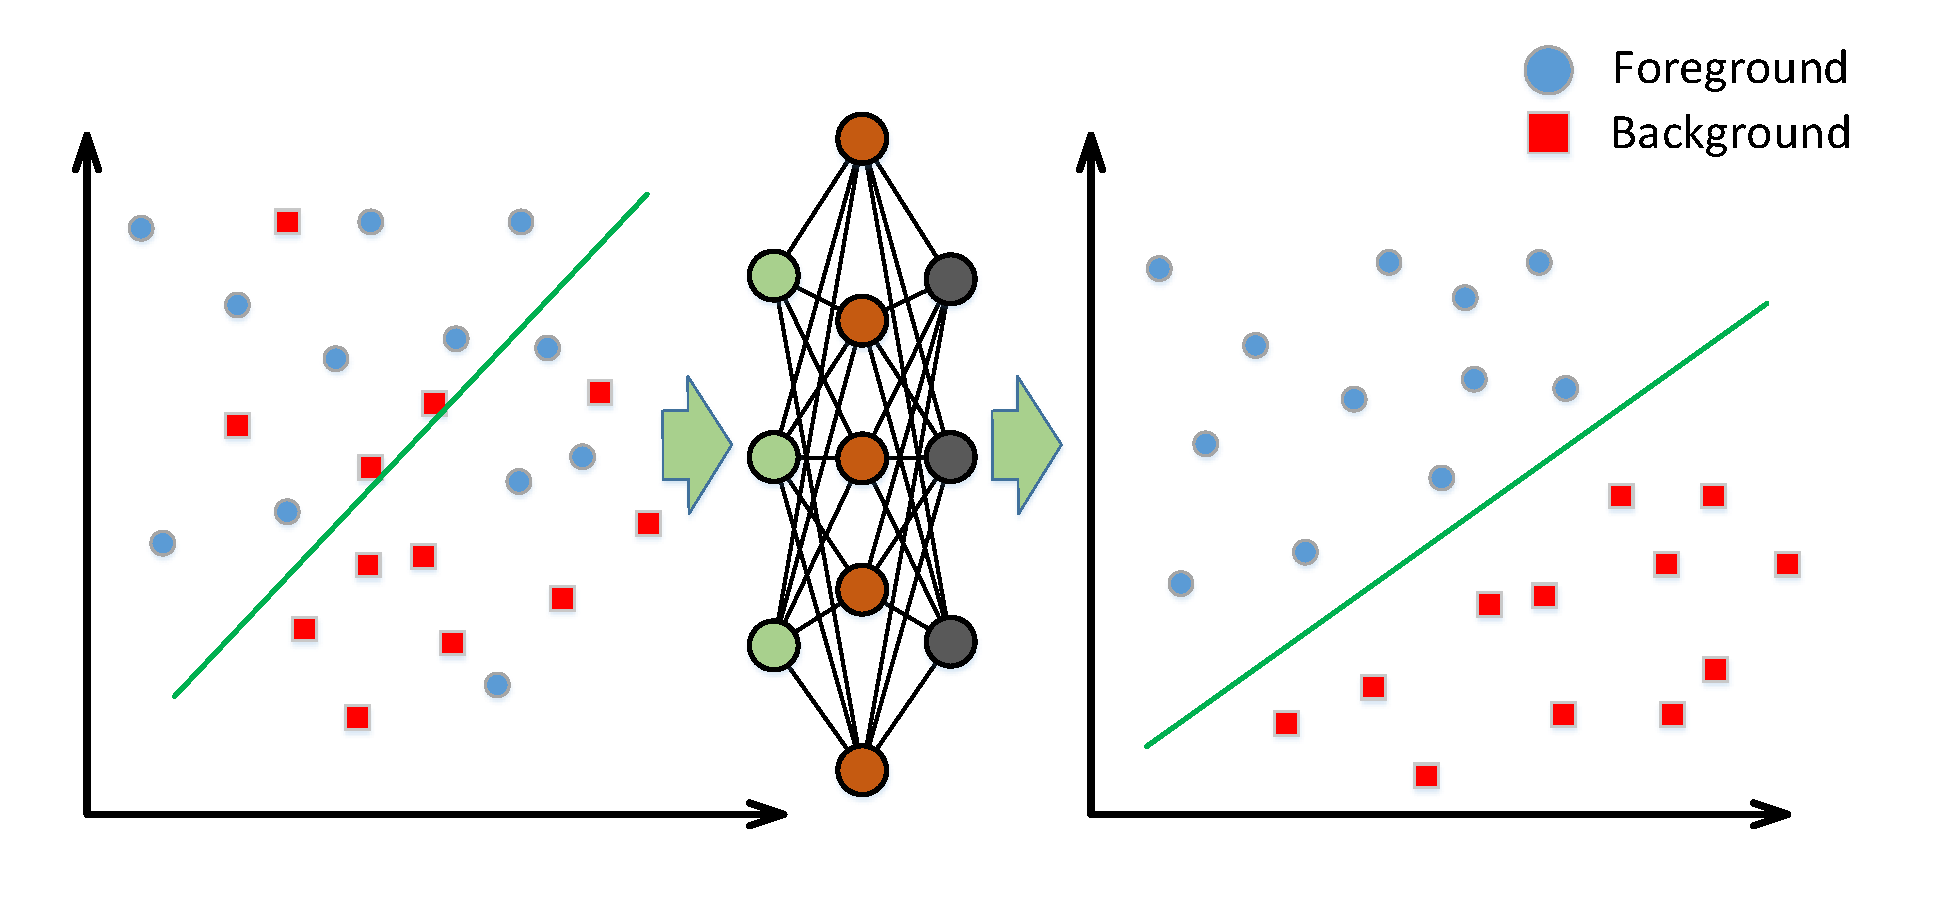
\includegraphics[width=\linewidth]{figure/fig1}
    % 图例里描述一下。
    \caption{Comparison of the original pixel variation, groundtruth and transformed variation. They are represented by the blue, red and green lines respectively.}
    \label{variation_chart}
\end{figure}
% It is hard to separate the foreground pixels from the background precisely in a time sequence.

%图例解释困难点
To give an intuitive understanding of the pixel variation, we plot the historical observations and the corresponding groundtruth of a single pixel in  \reffig{variation_chart}.
% with the X axis showing their range of variation and the Y axis representing the time. 
As we can see, there are several lines in three colors: blue, red and green. 
The blue line consists of original observations, representing a piece of pixel variation. 
Accordingly, the red line is made of the groundtruth data, corresponding to the observations from the blue one.  
And the green line consists of the outputs of the proposed approach which represents the transformed variation. 

%In practice, foreground detection is to produce a prediction curve, which is as near as possible to the groundtruth carve, by given the pixel variation carve. 

%传统方法的问题
Previous methods have good performance when background and foreground observations are significantly different and the backgrounds are normally static. 
While in fact, backgrounds can be rather turbulent and dynamic due to the complexity and diversity of natural scenes. 
Especially when illumination and camouflage are involved, background and foreground observations are easily confused and mixed up. 

%图例说明可能面临的挑战
For example, in \reffig{variation_chart}, it is noticeable that some foreground observations on the blue line share the same or similar value with background ones. 
In this case, popular methods will inevitably yield some sticky moments when separating the pixels in the blue line. 
Statistical methods, for instance, are no longer valid, because they only focus on establishing a statistical model for the background, while having little or no concern for the temporal coherence of these observations. 
In other words, despite knowing that pixels from the background share some common patterns of variation in a temporal sequence, they still let the order information of sequential images be ignored. 
%variation transformation 介绍。
%In this paper, a novel framework of pixel variation transformation is proposed. %用framework代替method?

Differring from existing methods, we decided to shift our attention from single pixel classification to variation transformation.
%the pixel variation is now regarded as a whole to safeguard the data integrity.
More specifically, a FCN is employed to learn patterns of pixel variations and mapping them into a new space where they are close to the groundtruth data.
The transformed variation is shown by the green line in \reffig{variation_chart}. 
%After thresholding, we can easily get the labels of each observation. 
%方法的好处是
The benefits are evident and can be clearly seen. 
It is hard to distinguish a foreground observation when its value is similar to the background ones. 
Classification on the transformed variation, however, is much more convenient and intuitive. 
With the strong learning ability of the FCN, we are able to learn the diverse variation patterns of background and foreground over a long period of time.
The variation patterns, in turn, contribute to the variation transformation where the value of each observation is adjusted according to its compatriot in time sequence.


%With the aid of deep learning method, the proposed approach can be effectively implemented.

% 公式表达
%And the definition of region searching method $G(x,y)$ is shown as follows:
%\begin{equation}
%    G(x,y) =  \mathop{\argmin}_{}{ \lVert I_t(m,n) - I_b(x,y) \rVert_{1}  } \quad  m,n \in x,y \pm R,
%\end{equation}

%where $x$ and $y$ is the location of pixels. And $I_t$ is the current frame, where $t$ is the
%time index.

%me
\section{Foreground Detection via Deep Variation Transformation}
\label{sec4}
In this section, details of the proposed approach are explained.
%
The pipeline of the proposed approach is shown in \reffig{flow_chart},
which can be divided into three parts.
%
First, the procedure generating pixel patches,
which are fed into the network for training as well as the description of pixel variation,
is introduced.
%
Then,
the architecture of the network, which is devised for transforming the variation of pixels' observations, is demonstrated.
%
Next,
a reverse procedure for the generation of training data is used to reconstruct the foreground image from the transformed results.
%
%We explain the production of the pixel patch, 
%which is a specific form of the pixel variation, and the architecture of our network. 
%

\begin{figure*}[!t] % FIGURE: figure/fig1 
\centering
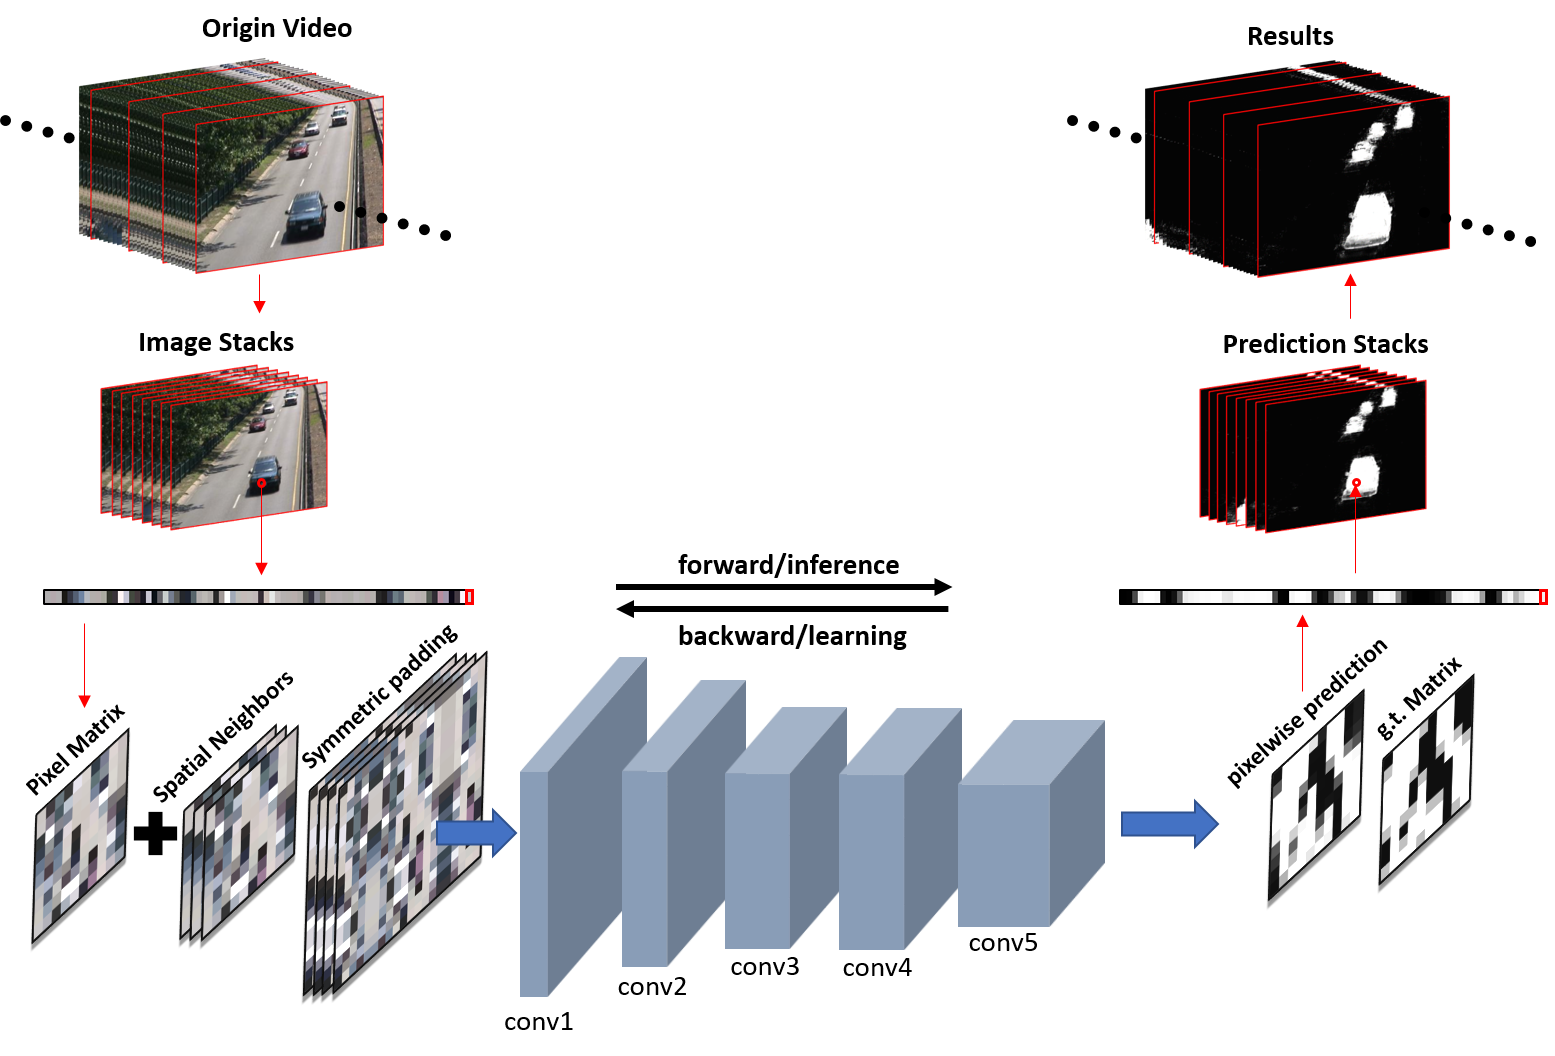
\includegraphics[width=\textwidth]{figure/fig2}
\DeclareGraphicsExtensions.
    \caption{ Original videos broken down into pixel patches for training of the FCN, which 
produces an efficient machine for end-to-end transformation learning.}
    \label{flow_chart}
\end{figure*}
% Firstly, we sample the input and ground truth images to generalize the pixel variations, 
% and reshape them into patches and feed them into the network with its spatial neighbors. 
% %
% After reassembling the patches into the complete output frame, 
% it is post-processed, yielding the final segmentation of the respective video frame.

\subsection*{Training Data Generation}
% 第一步是对原视频进行采样
%从描述事实开始
Fundamentally, 
background subtraction is a classification of pixels' observations in time sequence.
% 我们的动机
In this work,
a deep learning network is utilized to learn the pattern of variations implied in the observations of pixels.
% 基于这个动机,我们是怎么做的
Therefore,
the training data fed into the network is a type of description of pixels' variation,
which are actually patches consisting of pixels' temporal observations.
%
In contrast, the output of the network is the probability of corresponding pixels belonging to foreground or background,
and the network is devised with an end-to-end architecture to transform the intensity of pixels to the probability of the category the pixels belong to.

% 用数学化的语言描述具体过程
Let us denote the frames in a video sequence as $\mathcal{I} = \{I_1, I_2, \cdots, I_T\}$,
where $\mathcal{I}$ denotes the set of frames and $T$ is the numbers of frames.
%
There are usually large numbers of frames in a particular video,
and the number of frames for different videos are also different.
%
In order to capture the global representation of pixel's variation,
the training frames are sampled from the whole frame sequence uniformly.
%
% Let us denote the frame sequence as $\mathcal{I} = \{I_1, I_2, \cdots, I_T\}$,
% where $\mathcal{I}$ is denoted as the set of frames and $T$ is the numbers of frames.
%
The uniform sampling procedure is shown as follows:
% 
% Given different videos, their numbers of frames are generally different. 
% In order to keep each piece of variation the same length,
% image stacks are sampled from the given videos before the pixel variations are extracted. 
% Let denote the frames sequence as:
% \begin{equation}
%     \mathcal{I} = \{I_1, I_2, \cdots, I_T\}, \\\\
% \end{equation}
% 
% And image stacks can be defined as follows: 
\begin{equation}
    \mathcal{I}^d = \mathcal{D}(\mathcal{I})=  \{I_1, I_{[2 \cdot \frac{T}{N}]}, \cdots, I_{[(N - 1) \cdot \frac{T}{N}]}, \}
\end{equation}
where $\mathcal{I}^d$ is the set of training frames,
$T$ the $N$ represent the frame numbers of the entire video and the training set respectively,
and $\mathcal{D}()$ denotes the sampling function.
% 
% 
% %
% 
% 
% 
% % 解释采样的细节
% where $I_t$ is the frame $t$ of the given video. 
% $T$ and $N$ represent respectively the totall number of the video frames and the number of image stacks. 
% For each video, we can produce multiple image stacks and choose one of them for the training. 
% In addition, we can get compact pixel variations, which contain more temporal information than the continuous pixel sequences, by using equal interval sampling. 

After sampling training frames,
the training patches, which are used as the input to the network, are captured.
%
The training patch is the description of the pixels' variation,
which is captured by reshaping the observations in a particular pixel into a square patch.
%
Since the patch can be captured from each pixel, 
a large number of training patches can be extracted with the training frames;
and each of these patches has $\frac{T}{N}$ pixels.
%
In addition, for each pixel included in a patch, a label of the foreground or background is needed for training.
%
Therefore,
the labeling patches, which are captured by a similar procedure in the ground truth frames,
are used as the output for training our network.
Our network is actually an end-to-end transformation from pixels to labels.
%
Mathematically, the generation procedure of training patches can be shown as follows:
\begin{equation}
    S_{x,y}(m,n) = \mathcal{C}(\mathcal{I}^d, R) = \mathcal{I}_{m \times R + n} (x,y),
    \label{eq_reshape}
\end{equation}
where $S_{x,y}(m,n)$ denotes the training patch extracted from the observations of pixel located at $(x,y)$,
$R$ is the user argument to control the radius of training patches
and $\mathcal{C}(\mathcal{I}^d, R)$ is the function to convert the observations of pixels to training patches.
% where the pixel patch is denoted as $S_{x,y}(m,n)$, at the pixel positionthe pixel position $(x,y)$. 
% And the parameter $R$ is the column and row of pixel patches. 
% the column and row of the pixel patch. 
% Observations are put into the $R\times R$ patch from top to bottom and left to right.
% To put it another way, the pixel patch is just a specific form of the pixel variation. 
% %Although the observation patch and the observation sequence belong to different forms of the pixel variation, they consist of the same components, and share the common temporal information from the pixel variation. 
% Since the pixel sequences are extracted from each pixel position, a large number of pixel patches can be extracted from only one single image stack, which promises sufficient training data for our network.
% 
% 
% Mathmatically,
% 
% 
% the labeling patches are also captured by the similar procedure in the groundtruth frames.
% %
% 
% 
% 
% the frames of ground truth are 
% 
% 
% which describe the variation of pixels' observations, are captured.
% %
% The pathces 
% 
% 
% % 第二步提取Pixel variation
% After the sampling process, a large number of observation sequences, or pixel variations, can be extracted from the chosen stack at each pixel position.
% Each of the pixel variation is a piece of temporal information which containing the changing patterns of background pixels. 
% And each of them is of fixed length $\cdot \frac{T}{N}$. 
% It is notable that observation sequences are extracted from individual pixel positions, which promises that sufficient training data can be obtained with only one image stack.
% 
% % 第三步变成矩阵形式,解释为什么要把variation 变形
% Our task is to provide an end-to-end transformation of pixel variations, based on the strong learning ability of FCNs. 
% However, vectors are not appropriate for the network training and learning. 
% Besides, we also hope pixel observations can be interacted with their further compatriots in temporal sequence. 
% Thus we reshape the variations into pixel patches as the input of our network. 
% A sample of the pixel patch is like this:
% \begin{equation}
%     S_{x,y}(m,n) = \mathcal{C}(\mathcal{I}^d, R) = \mathcal{I}_{m \times R + n} (x,y),
% \end{equation}
% where the pixel patch is denoted as $S_{x,y}(m,n)$, at the pixel positionthe pixel position $(x,y)$. 
% And the parameter $R$ is the column and row of pixel patches. 
% the column and row of the pixel patch. 
% Observations are put into the $R\times R$ patch from top to bottom and left to right.
% To put it another way, the pixel patch is just a specific form of the pixel variation. 
% %Although the observation patch and the observation sequence belong to different forms of the pixel variation, they consist of the same components, and share the common temporal information from the pixel variation. 
% Since the pixel sequences are extracted from each pixel position, a large number of pixel patches can be extracted from only one single image stack, which promises sufficient training data for our network.

%第四步空间近邻随机采样。
It is generally accepted that a pixel is not independent but related to its neighborhood,
and similar neighboring pixels share similar variations.
%
Therefore,
spatial information should benefit from learning the pattern of pixels' variation.
%
With this motivation,
several training patches extracted from neighboring pixels are combined to improve the efficiency of the proposed approach.
%
In the experiments, three training patches are combined as follows:
\begin{equation}
    S_{x,y}(m,n) = \mathcal{C}o(S_{x,y}(m,n), S_{x', y'}(m,n), S_{x'', y ''}(m, n)),
\end{equation}
where $\mathcal{C}o$ represents the concatenation process on the third dimension.
And neighboring patches are at pixel position $(x',y')$ and $(x'',y'')$ respectively.
% Ii is generally accepted that neighboring background pixels share a similar temporal distribution.
% %In other words, there are some clues hidden in pixels' spatial neighbors. 
% In order to benefit from the spatial context, we concatenate the pixel patch with 2 neighboring pixel patches, 
% 
% which are randomly selected in the 8-connected neighborhood of each pixel position. 
% The input patch of our network is defined as:
% \begin{equation}
%     S_{x,y}(m,n) = \mathcal{C}o(S_{x,y}(m,n), S_{x', y'}(m,n), S_{x'', y ''}(m, n)),
% \end{equation}
% where the $\mathcal{C}o$ represents the concatenation process on the third dimension.
% And neighboring patches are at pixel position $(x',y')$ and $(x'',y'')$ respectively.
% 
%In the previous steps, original videos are broken down into pixel patches which contain abundant background information. 

\subsection*{Network Architecture and Variation Transformation}
% 先描述动机
As we mentioned above,
the main purpose of our DPVTL algorithm is the transformation between the sequence of pixels' observations with possibility of pixels belonging to foreground or background.
% the main purpose of our DPVTL is trying to transform the sequence of pixels' observations 
% into another space where the observations are easier classified.
% 分析问题,提出解决的方案,要用数学化的形式
Therefore,
our network entails learning a mapping from the input observations of pixels $s \in \mathcal{S}$ 
to the probability $p \in \mathcal{P}$ of the corresponding pixel belonging to foreground or background.
%
An end-to-end architecture network is proposed to transform the observations of pixels to a new space which is close to labels, as shown in \reffig{flow_chart}.
%
Mathematically, the training procedure is as follows:
\begin{equation}
    \begin{split}
        \mathcal{P}(m,n) & = f_{\theta_N} ( f_{\theta_{N - 1}} ( \cdots f_{\theta_1} ( \mathcal{S}(m,n)) \cdots  ) )  \\
          & = f_{ \prod_{n=1}^{N}\theta_n   }^n(\mathcal{S}(m,n)),
    \end{split}
\end{equation}
where $\mathcal{P}(x,y)$ is the probability, $\mathcal{S}(m,n)$ is the input patch of the network and $f_{\theta_i}$ represents different layers of the network.
% where, $S'(m,n)$ is the prediction of the network, and the forward computation at each layer of the network is represented by $f_{\theta_N}$. The symmetric padding process is denoted as $Pad$, where we have lost none of the pixel information to make the output $S'(m,n)$ the same size as the pixel patch $S(m,n)$. 
% Another advantage of symmetric padding is that the order information still remains.

For the loss function, Sigmoid Cross Entropy (SCE) loss is used, which helps address the learning slowdown. 
The formulation is as follows:
\begin{equation}
    \begin{split}
         \mathcal{L}(S'(x,y),& S^{gt}(x,y))  =  \sum_{x=1}^{m}\sum_{y=1}^{n} S^{gt}(x,y) log(Sig(S'(x,y)))  \\
        & + (1 - S^{gt}(x,y)) log(1 - Sig(S'(x,y))), 
    \end{split}
\end{equation}
\begin{equation}
       Sig(x) =\frac{1}{1+e^{-x}},
\end{equation}
where $S^{gt}(x,y)$ denotes the groundtruth patch which is given by the corresponding groundtruth stack, and $Sig$ represents the sigmoid function. 
SCE is calculated between the transformed patches and the corresponding groundtruth patches. 
Boundaries of moving objects and pixels that are out of the region of interest are not taken into account in the cost function.
Finally, we get the transformed variation through the FCN, which is much easier for classification. 

% 描述网络结构
%The network used in this work is devised as an end-to-end architecture XXX
The architecture of our FCN for foreground detection is illustrated in \reffig{flow_chart}. 
The proposed FCN contains 6 convolutional layers without pooling, and the filter size of the first five layers is set to $3\times 3$, compared to the last convolutional layer which has a filter size of $1\times 1$. 
We use the Rectified Linear Unit (ReLU) as the activation function after first three convolutional layers,
and the Sigmoid Cross Entropy loss function is applied to measures the performance of our network after the last convolutional layer. 
We do not use any other adjustment in our network training and the experimental results prove that the proposed approach is feasible and very effective.
After the thresholding calculations, our experiments show that a randomly initialized FCNs, 
trained end-to-end on feature learning can achieve state-of-the-art performance without any extra optimization mechanism.



% 
% 
% As shown in the \reffig{flow_chart},
% %
% The input of network is the training patches $S(m,n)$ extracted from different pixels
% and the output of network is the labeled patches captured from Groundtruth frames.
% %
% The training procedure is the transformation from the training patches to the labelling patches,
% which is shown as follows:
% % 
% % the architecture of network 
% % 
% % Correspondingly, the groundtruth patches are obtained in a similar way as the input ones, except the concatenation process, as shown in the \reffig{flow_chart}. 
% % Both of them are fed into the network for training to find a end-to-end transformation at each pixel position. 
% % However, the size of feature maps will shrink quickly during forward computation. 
% % In preprocessing, we borrow the idea from Image Semantic Segmentation \cite{Shelhamer2017fcn}, padding the input patches before the training. 
% % After the forward computing, observations in input patches are mapped into a new space where they can be easily classified by thresholding. 
% % The transformed pixel patch is defined as:
% \begin{equation}
%     \begin{split}
%         S'(m,n) & = f_{\theta_N} ( f_{\theta_{N - 1}} ( \cdots f_{\theta_1} (Pad(S(m,n))) \cdots  ) )  \\
%           & = f_{ \prod_{n=1}^{N}\theta_n   }^n(S(m,n)),
%     \end{split}
% \end{equation}

\subsection{Foreground Detection}
%As shown in the \reffig{flow_chart}, 
After the transformation from observations to the probability of belonging to foreground or background,
the foreground is detected from the final binary mask.
%
During the transformation,
the pixel patches are fed into the network and transformed into the probability patches,
which are compared with a threshold $T_r$ for classification and then used to reconstruct the foreground to obtain the final results.
%
Comparison with a threshold can be mathematically shown as:
\begin{equation}
    \mathcal{M}(x,y) = g(T_f, \mathcal{C}^{-1}(S'(x,y), R)),
\end{equation}
where the $\mathcal{M}(x,y)$ is the final binary mask.
%
$S'(x,y)$ is the probability of patches output by the network,
$\mathcal{C}^{-1}$ is the reverse of the reshape procedure shown in \refeq{eq_reshape} and $R$ is the parameter for the reversing reshape procedure.
%
$T_f$ is the threshold given by a user and $g()$ is the thresholding function shown in \refeq{piecewise_fg}.
% Then the reverse procedure of \refeq{eq_reshape}
% 
% used to reconstruct the foreground image for the final results.
% %
% 
% 
% The network devised in proposed approach 
% 
% 
% Then, the prediction maps can be reconstructed from the prediction patches.
% %
% Then a global threshold $T_r$ is set for each transformed observation in order to map them to $\{0,1\}$. 
% %
% The threshold function is given by
\begin{equation}
    \label{piecewise_fg}
    g(x,y) =
 \begin{cases}
  1,  \quad x < y       \\
  0,  \quad otherwise   \\
\end{cases},
\end{equation}
%
%where the $M$ denotes the final foreground map given by our DPVTL model.

%Here we make a detailed introduction to the deep learning model we used and explain why we choose it.

%Different with CNNs, FCNs utilize convolutional layers with $1\times 1$ kernels to take the place of fully connected layers, which provide several benefits. First and foremost, the size of output is adjustable in FCNs, which allows an end-to-end mapping of input patches and prediction patches at each pixel position. 
%We hope to determine the label of an observation through the comparison of its compatriot in time sequence. 
%There is one more point I ought to touch on, that since the feature maps are no longer needed to be converted into vectors, spatial information can be retained. 
%The last but not the least, FCNs have been used in sematic segmentation and researchers found FCNs have a strong learning ability which won't lose to the traditional ones. 
%Meanwhile, it's also a highly efficient computation model. 
%Based on above-mentioned factors, FCN is designed as the alternative network architecture in this paper. 


\section{Experiments}
\label{sec5}
In this section, we describe comprehensive experiments to evaluate the performance of the proposed approach on the CDnet 2014 benchmark\cite{CDN2014} and CAMO-UOW\cite{CAMO}.
%
CDnet is the largest dataset for foreground detection as far as we know, containing 11 categories with several complex challenging scenes, such as Dynamic Background, Camera Jitter, Shadow, Night Videos, PTZ and so on. 
The CAMO-UOW is a challenging benchmark for camouflaged foreground detection, containing 10 high resolution videos. 
For each video, one or two persons appear in the scene with clothes having color similar to the background.

The proposed approach is compared with several existing traditional state-of-the-art foreground detection algorithms, including IUTIS-5\cite{Bianco2017TEC}, SuBSENSE\cite{St-Charles2015SuBSENSE}, WeSamBE\cite{Jiang2017WeSamBE}, sharable GMM the SharedModel\cite{Chen2015SharedModel}, word-dictionaries-based method like PAWCS\cite{Charles2015PAWCS}, SemanticBGS\cite{Braham2017Semantic} and AAPSA\cite{RAMIREZALONSO2016990}.
Moreover, two deep learning based algorithms are also compared with the proposed approach, including DeepBS\cite{Babaee2017deep}, and DBMF\cite{Yang2018DBMF}. 
The results of the compared algorithms are captured by the implementation provided by the authors.
% \textcolor{red}{All the results of compared algorithms are provided by authors.}

For comparison, the F-measure Space (Fm) is used for evaluation. 
Fm is a general international standard in foreground detection which measures the segmentation accuracy by considering both recall and precision. 
The definition of Fm is as follows:
\begin{equation}
Fm= \frac{2\times precision \times recall}{precision + recall} = \frac{2TP}{2TP+FN+FP},
\end{equation}
% 
% 
% \begin{equation}
%     F=\frac{precision \dot recall}{precision - recall}  = \frac{2TP}{2TP+FN+FP},
% \end{equation}
%
where TP, FP, and FN are true positives, false positives, and false negatives respectively, computed on the pixels of all the test frames for each video. 

\begin{figure*}[!t]	\centering
    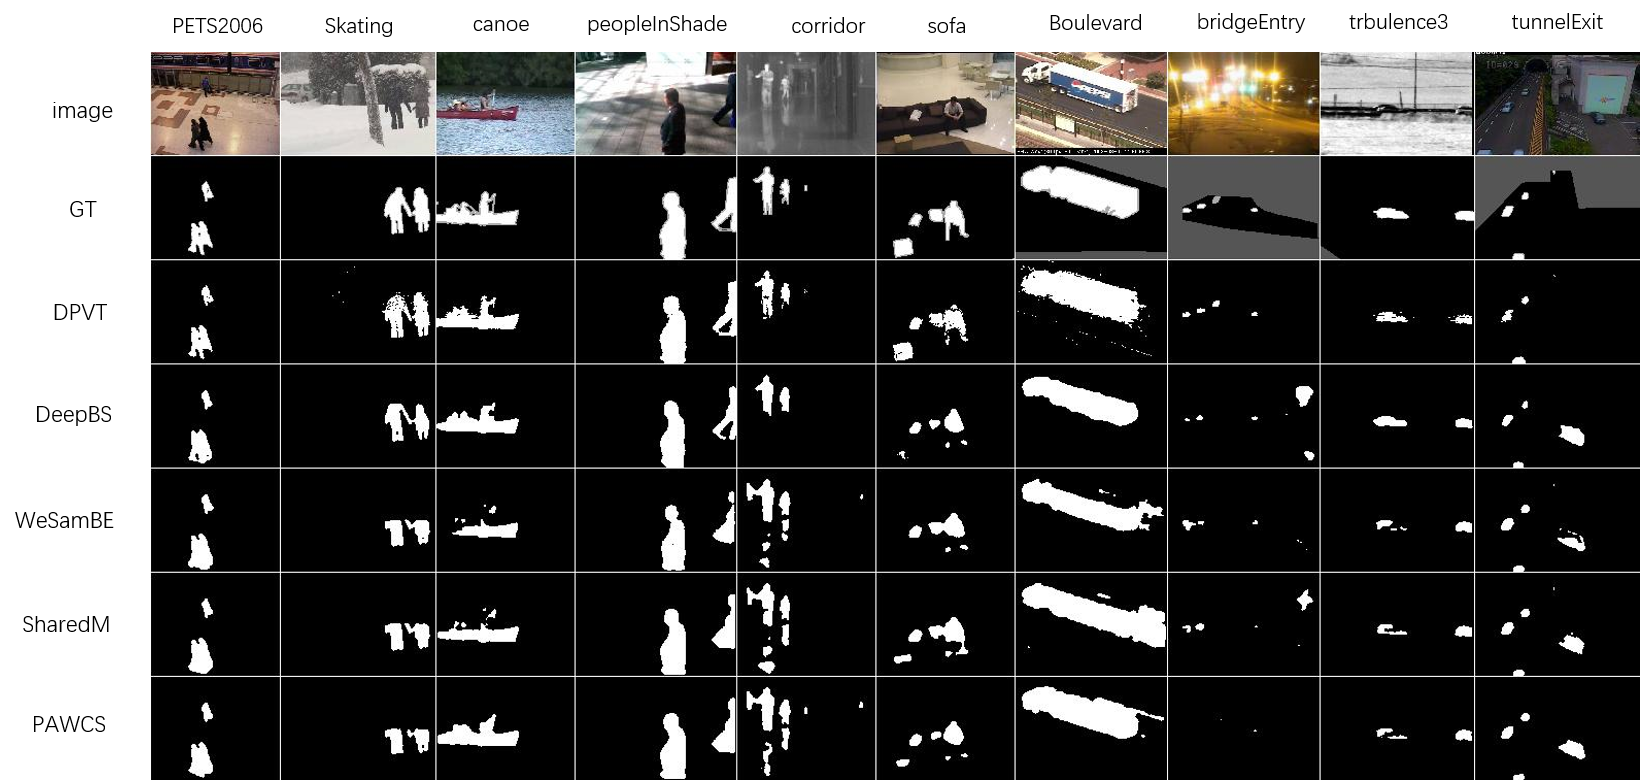
\includegraphics[width=\textwidth]{figure/fig3}
\DeclareGraphicsExtensions.
    \caption{The qualitative evaluation of the proposed method. All the results is followed in the CDnet 2014.}
    \label{results_chart}
\end{figure*}

Quantitative and qualitative comparisons are shown in \reftab{tab1} and  \reffig{results_chart} respectively. 
To keep the length of this paper reasonable, only several typical videos are selected for the qualitative comparisons and discussion. 
In the dynamic background scene, the video ``canoe'' is a typical challenging video which includes a large area of rippling water. 
The main challenge comes from the dynamic background, in which it is hard to describe the background by a single image. 
For this condition, since traditional foreground detection methods such as the SharedModel and the WeSamBE cannot describe the complex dynamical background, they fail to detect the people on the boat, as shown in \reffig{results_chart}. 
Besides, the detected moving objects of the SharedModel are not accurate in the boundary due to the utilization of texture features. 
In contrast, benefiting from the strong learning ability of Deep Learning networks, DeepBS successfully detects the people. 
Unfortunately, since the DeepBS ignores the fact that a single background is not enough to describe the dynamic background, even this algorithm suffers from poor detection of the boat shape. 
In contrast, the proposed approach performs better than others in this scene, since the essence of foreground detection is considered as a binary classification of pixels' observation over a time sequence. 
Based on this insight, the FCN network focuses on learning the patterns of pixel variation rather than a static background image.
Thus the proposed approach achieves promising performance for the canoe video.



As for the case of the shadow scene, ``peopleInShade'' is a typical example with prevalent hard and soft shadows. 
For traditional approaches, these shadow regions are usually segmented as foreground since they also movie with the objects. 
Therefore, traditional methods like PAWCS, WeSamBE and SharedModel falsely segment part of shadows as moving objects. 
In addition, the foreground provided by IUTIS-5 is incomplete on part of the pedestrian's body due to the interference of shades, 
because of the severe dependency on texture features. 
On the other hand, DeepBS performs well for this video benefiting from the utilization of CNN. 
However, the shape of pedestrians are slightly deformed as a result of the patch-wise processing in CNN. 
In contrast, since our DPVL focusses on learning the pattern of pixels' variation in the shadow regions, 
the proposed approach successfully segments the shadow part as the background and achieves the highest performance in the category of shadow scene.

In the video ``corridor'' among the Thermal scene, there is no color information since the videos are obtained through a Thermal camera. 
Moreover, moving objects in these videos are exceedingly fuzzy and unclear, which is the main challenge for this category. 
WeSamBE, SharedModel and PAWCS successfully detect the target objects, because of a stable background in this indoor video. 
However, they fail to remove the reflections since their modeling ability has already reached a limit under the extreme condition of the thermal map. 
DeepBS, by contrast, succeeds in eliminating most of the reflections. 
Meanwhile, moving objects are also clearly divided from the background thanks to the strong modeling ability of CNN. 
However, due to the dependency of the edge feature, a small object was missed in the detection result. 
Fortunately, the proposed approach utilizes the pattern of pixels' variation, which is theoretically effective even in observations without color information. 
Consequently, our DPVTL performs much better than other algorithms, with most parts of the shadow being removed and the segmentation results become more accurate.

% \begin{table}[tab1]
\begin{table*}[!t]				% TABLE
\centering
\caption{Performance comparison of the proposed approach and some state-of-the-art algorithms on the video sequences from different categories in CDnet 2014. For each video, 100 frames were taken for training our FCN.}
\label{tab1}
\begin{tabular}{lllllllllllll}
\hline
Videos      & baseline & dyna.bg & cam.jitter & int.obj.m & shadow & thermal & bad.weat & low f.rate & night vid. & PTZ    & turbul. & overall \\ \hline
DeepBS\cite{Babaee2017deep}      & 0.9580   & 0.8761  & 0.8990     & 0.6097    & 0.9304 & 0.7583  & 0.8647   & 0.5900     & 0.6359     & 0.3306 & 0.8993  & 0.7458  \\
IUTIS-5\cite{Bianco2017TEC}     & 0.9567   & 0.8902  & 0.8332     & 0.7296    & 0.9084 & 0.8303  & 0.8289   & \textbf{0.7911}     & 0.5132     & 0.4703 & 0.8507  & 0.7717  \\
FTSG\cite{Wang2014FTSG}        & 0.9330   & 0.8792  & 0.7513     & 0.7891    & 0.8832 & 0.7768  & 0.8228   & 0.6259     & 0.5130     & 0.3241 & 0.7127  & 0.7283  \\
AAPSA\cite{RAMIREZALONSO2016990}       & 0.9183   & 0.6706  & 0.7207     & 0.5098    & 0.7953 & 0.7030  & 0.7742   & 0.4942     & 0.4161     & 0.3302 & 0.4643  & 0.6179  \\
CwisarDH\cite{Gregorio2014CwisarDH}    & 0.9145   & 0.8274  & 0.7886     & 0.5753    & 0.8581 & 0.7866  & 0.6837   & 0.6406     & 0.3735     & 0.3218 & 0.7227  & 0.6812  \\
PAWCS\cite{Charles2015PAWCS}       & 0.9397   & 0.8938  & 0.8137     & 0.7764    & 0.8934 & 0.8324  & 0.8059   & 0.6433     & 0.4171     & 0.4450 & 0.7667  & 0.7403  \\
SuBSENSE\cite{St-Charles2015SuBSENSE}    & 0.9503   & 0.8177  & 0.8152     & 0.6569    & 0.8986 & 0.8171  & 0.8594   & 0.6594     & 0.4918     & 0.3894 & 0.8423  & 0.7408  \\
SemanticBGS\cite{Braham2017Semantic} & 0.9604   & \textbf{0.9489}  & 0.8388     & 0.7878    & 0.9244 & 0.8219  & 0.8260   & 0.7888     & 0.5014     & 0.5673 & 0.6921  & 0.7892  \\
MBS\cite{Multimode_Background_Subtraction}         & 0.9287   & 0.7915  & 0.8367     & 0.7568    & 0.8262 & 0.8194  & 0.7980   & 0.6350     & 0.5158     & 0.5520 & 0.5858  & 0.7288  \\
WeSamBE\cite{2017_TCSVT_BG_7938679}     & 0.9413   & 0.7440  & 0.7976     & 0.7392    & 0.8999 & 0.7962  & 0.8608   & 0.6602     & 0.5929     & 0.3844 & 0.7737  & 0.7446  \\
ShareM\cite{2015_ICME_ShareModel}      & 0.9522   & 0.8222  & 0.8141     & 0.6727    & 0.8898 & 0.8319  & 0.8480   & 0.7286     & 0.5419     & 0.3860 & 0.7339  & 0.7474  \\
GMM\cite{Zivkovic2004}         & 0.8245   & 0.633   & 0.5969     & 0.5207    & 0.7370 & 0.6621  & 0.7380   & 0.5373     & 0.4097     & 0.1522 & 0.4663  & 0.5707  \\
RMoG\cite{Varadarajan2013}        & 0.7848   & 0.7352  & 0.7010     & 0.5431    & 0.7212 & 0.4788  & 0.6826   & 0.5312     & 0.4265     & 0.2470 & 0.4578  & 0.5735  \\ \hline
DPVT        & \textbf{0.9811}   & 0.9329  & \textbf{0.9014}     & \textbf{0.9595}    & \textbf{0.9467} & \textbf{0.9479}  & \textbf{0.8780}   & 0.7818     & \textbf{0.7737}     & \textbf{0.5957} & \textbf{0.9034}  & \textbf{0.8789} \\ \hline
\end{tabular}
\end{table*}

\begin{table*}[!t]
\centering
\caption{Performance comparison of the proposed approach and some classical methods and deep-based method DBMF. For each video, 64 frames were taken for training our FCN.}
\label{tab2}
\begin{tabular}{llllllll}
\hline
Methods  & highway & office & Pedestrians & PETS2006 & Fall   & sofa   & overall \\ \hline
GMM\cite{Stauffer1999}      & 0.5788  & 0.2338 & 0.5202      & 0.6011   & 0.8026 & 0.5225 & 0.5432  \\
CodeBook\cite{WU2010739} & 0.8356  & 0.5939 & 0.7293      & 0.7808   & 0.3921 & 0.8149 & 0.6911  \\
ViBe\cite{Barnich2011_2011_TIP}     & 0.7535  & 0.6676 & 0.8367      & 0.6668   & 0.6829 & 0.4298 & 0.6729  \\
PBAS\cite{Hofmann2012Background}     & 0.8071  & 0.6839 & 0.7902      & 0.7280   & 0.3420 & 0.5768 & 0.6547  \\
P2M\cite{Yang2016P2M}      & 0.9160  & 0.3849 & 0.9121      & 0.7322   & 0.5819 & 0.4352 & 0.6604  \\
DBMF\cite{Yang2018DBMF}     & 0.9412  & 0.9236 & 0.8394      & 0.9059   & 0.8203 & 0.8645 & 0.8824  \\ \hline
DPVT     & \textbf{0.9888}  & \textbf{0.9819} & \textbf{0.9728}      & \textbf{0.9808}   & \textbf{0.9394} & \textbf{0.9333} & \textbf{0.9662}  \\ \hline
\end{tabular}
\end{table*}

    
    \begin{table*}[!t]
\centering
\caption{Performance comparison of the proposed approach and some state-of-the-art algorithms on video sequences from different categories in CAMO-UOW.}
\label{tab3}
\begin{tabular}{lllllllllll}
\hline
Methods  & MOG2\cite{ZIVKOVIC2006773} & FCI\cite{Baf2008FCI}  & LBA-SOM\cite{LBA-SOM2008} & PBAS & SuBSENSE & ML-BGS\cite{ML-BGS2007} & DECOLOR\cite{DECOLOR2013}       & COROLA\cite{SHAKERI201628} & FWFC\cite{Li2018CAMO}          & DPVT          \\ \hline
Video 1  & 0.79 & 0.88 & 0.8     & 0.9  & 0.89     & 0.89   & 0.92          & 0.8    & 0.94 & \textbf{0.96} \\
Video 2  & 0.82 & 0.79 & 0.8     & 0.82 & 0.88     & 0.8    & 0.83          & 0.58   & 0.96          & \textbf{0.98} \\
Video 3  & 0.88 & 0.86 & 0.85    & 0.91 & 0.9      & 0.8    & 0.9           & 0.82   & 0.94 & \textbf{0.95} \\
Video 4  & 0.89 & 0.9  & 0.76    & 0.93 & 0.78     & 0.88   & 0.95          & 0.87   & 0.94          & \textbf{0.98} \\
Video 5  & 0.84 & 0.86 & 0.82    & 0.83 & 0.82     & 0.8    & 0.82          & 0.75   & 0.91          & \textbf{0.98} \\
Video 6  & 0.93 & 0.87 & 0.77    & 0.95 & 0.92     & 0.95   & 0.97	      & 0.72   & 0.94          & \textbf{0.98}  \\
Video 7  & 0.76 & 0.83 & 0.88    & 0.91 & 0.87     & 0.79   & 0.91          & 0.83   & 0.96          & \textbf{0.99} \\
Video 8  & 0.83 & 0.87 & 0.85    & 0.87 & 0.93     & 0.86   & 0.86          & 0.68   & \textbf{0.96}          & \textbf{0.96} \\
Video 9  & 0.89 & 0.9  & 0.87    & 0.84 & 0.92     & 0.87   & 0.86          & 0.78   & 0.88          & \textbf{0.99} \\
Video 10 & 0.89 & 0.86 & 0.89    & 0.91 & 0.92     & 0.9    & 0.94          & 0.85   & 0.96          & \textbf{0.97} \\ \hline
average  & 0.85 & 0.86 & 0.83    & 0.89 & 0.88     & 0.85   & 0.90          & 0.77   & 0.94          & \textbf{0.97} \\ \hline
\end{tabular}
\end{table*}




The quantitative evaluation of the proposed approach on CDnet 2014 is shown in \reftab{tab1}. 
It can be seen that the proposed approach significantly outperforms all of the compared state-of-the-art algorithms in most of the complex scenes and achieves 11.37\% gain in FM over the second one on the whole dataset. 
%
Moreover,
since DBMF only published their results in several specific videos instead of the whole dataset,
the proposed approach was also ran in these videos to compare with DBMF with the results shown in Table 2.
This also demonstrates the superiority of the proposed approach.
% \textcolor{red}{Moreover, in order to compare the proposed approach with the DBMF, which is also based on deep learning and only publish their results in  specific videos. 
% The proposed approach has also ran in these videos and the results are shown in Table 2. 
% Again, the proposed approach has noticeably better performance than the DBMF and some other classical background approaches.}

As shown in \reftab{tab1} and \reftab{tab2}, previous deep learning based methods like DeepBS and DBMF achieve good performance. 
From our perspective, this good performance can be attributed to the stronger modeling ability and learning adaptation of CNN and FCN. 
However, the proposed approach utilizes pixel variations in a temporal sequence rather than low-level static features such as color, edges and textures, which give us the ability to avoid the shortcomings of the background models. 
Consequently, the proposed approach produces considerably better results, with improvement over 17.85\% in FM metrics compared to DeepBS and over 9.50\% compared to DBMF.

The evaluation of the proposed approach in CAMO-UOW dataset is shown in \reftab{tab3}. 
Unlike the CDnet dataset, the videos of CAMO-UOW dataset are specially proposed for moving objects with camouflage, which is the main challenge of this dataset. 
As shown in \reftab{tab3}, the proposed approach achieves better performance compared to its competitions, 
with an average F-measure of 0.97, compared to values between 0.77 and 0.94 for other methods. 
Therefore, it is fair to say that the proposed approach performs better compared to the state-of-the-art.


In the CAMO-UOW dataset, target objects have similar color and textures as the background. This creates many difficulties and obstacles for traditional methods. 
However, our FCN is a powerful Neural Network model which is good at capturing the non-linearities of the manifold of pixel variations. 


All of the experiments of the proposed method were implemented in Matlab and run on a computer with Nvidia Tasla K80 GPU with all images kept at their original resolution. 
For each video in CDnet 2014, 100 training frames are extracted to produce the image patch. 
It should be noted that the 100 frames only account for less than 10\% of total Groundtruth in CDnet 2014. 
In contrast, 90\% of data was used as training samples in DBMF, which suggests that the proposed approach achieves better performance with limited training frames. 
Considering that videos in CAMO-UOW have fewer frames, we reduced the number of training frames to 64 for each video. 
During the experiments, the training and testing sets are completely separated. 
More specifically, our FCN network is randomly initialized. 
We train the network with mini-batches of size 200, and a learning rate of $\alpha  = 1 \times 10^{{−3}}$ over 20 epochs. 
The last threshold $R$ is set to 0.6.


% \begin{table}[!t]				% TABLE
%     \caption{The example of latex table}
% \label{tab_FBMS_nobk}
% \centering
%     \begin{tabular}{|l@{  }c@{  }c@{  }cc@{  }c@{  }c@{  }c|}
% \hline
%      \multirow{2}{*}{Videos} & \multicolumn{3}{c}{$\text{IFB}_{nobk}$} &  & \multicolumn{3}{c|}{IFB} \\
%     \cline{2-4} \cline{6-8}
%        & Re &Pr & Fm &  &  Re & Pr & Fm  \\
% \hline
% cats03          &   (\textbf{0.9472} ,\   &  0.5428 ,\  &   0.6901 )   &  &    (0.9063 ,\	 &  \textbf{0.7955} ,\	 &  \textbf{0.8473} )   \\
% bear01          &   (\textbf{0.9854} ,\   &  0.4806 ,\  &   0.6461 )   &  &    (0.8695 ,\	 &  \textbf{0.8673} ,\	 &  \textbf{0.8684} )   \\
% rabbits01       &   (\textbf{0.9530} ,\   &  0.4433 ,\  &   0.6051 )   &  &    (0.9510 ,\	 &  \textbf{0.8730} ,\	 &  \textbf{0.9103} )   \\
% cars5           &   (\textbf{0.9887} ,\   &  0.3693 ,\  &   0.5378 )   &  &    (0.9437 ,\	 &  \textbf{0.7108} ,\	 &  \textbf{0.8109} )   \\
% tennis          &   (\textbf{0.9364} ,\   &  0.4558 ,\  &   0.6132 )   &  &    (0.8808 ,\	 &  \textbf{0.7345} ,\	 &  \textbf{0.8010} )   \\
% farm01          &   (\textbf{0.9887} ,\   &  0.3897 ,\  &   0.5591 )   &  &    (0.8954 ,\	 &  \textbf{0.7462} ,\	 &  \textbf{0.8140} )   \\
% \hline                                                                                                           
% Average         &   (\textbf{0.9666} ,\   &  0.4469 ,\  &   0.6086 )   &  &    (0.9078 ,\    &  \textbf{0.7879} ,\   &  \textbf{0.8420} )   \\
% \hline
% \end{tabular}
% \end{table}

% Videos & GBSSP\cite{Lim2014_2014_ECCV} & calMoSeg\cite{2016_ECCV_Bideau2016}  & MLayer\cite{2017_ICCV_zhu2017multilayer}  & $\text{IFB}_{SU}$ & $\text{IFB}_{KA}$ & $\text{IFB}_{SI}$ & Videos & GBSSP\cite{Lim2014_2014_ECCV} & calMoSeg\cite{2016_ECCV_Bideau2016} & MLayer\cite{2017_ICCV_zhu2017multilayer}  &  $\text{IFB}_{SU}$ &  $\text{IFB}_{KA}$  &  $\text{IFB}_{SI}$  \\




\section{Conclusion}
\label{sec6}
In this paper, we proposed a novel foreground detection approach based on our proposed variation transformation learning.
%
Transformation learning focused on learning a transformation from pixel variations to the probability of pixels belonging to the foreground or background.
%
The global variation patterns of pixel observation is learned for better classification of pixels.
%
In particular, a FCN network and a novel variation transformation learning framework is proposed to efficiently combine the temporal coherence and distribution information of pixels over a long period of time. 
%
Comparisons with other traditional and deep learning methods shows that our DPVTL algorithm significantly improves performance on several challenging scenes.
%The future work will be focused on improving the DPVTL in terms of network architecture updating and integration of local spatial coherence.

% \section{Conclusions}
% In this paper,
% we proposed the IFB framework for foreground detection for the case of a freely moving camera.
% Unlike previous work in which attempts were made to improve the accuracy of the estimation of motion,
% our IFB focuses on integrating rough foreground and background cues for foreground segmentation.
% In particular, 
% foreground cues are detected by a GMM model with the estimation of background motion,
% while background cues are captured from spatio-temporal features filtered by homography transformation,
% where the SURF\cite{2006_SURF}, KAZE\cite{2012_KAZE}, SIFT\cite{lowe2004distinctive} features are used as examples.
% % the geometric constraints between the SIFT features.
% Then, super-pixels under multiple levels are utilized to integrate these cues.
% The efficiency of IFB results from the complementarity between foreground and background cues.
% The accuracy of the proposed approach is improved though the utilization of super-pixels under multiple levels.
% A comprehensive experiment to compare our results with the state-of-the-art shows the efficiency of our framework and points to its potential for use in practical applications.
% 


\ifCLASSOPTIONcaptionsoff
  \newpage
\fi

\bibliographystyle{IEEEtran}  
\bibliography{ref}  


\end{document}
